\section{Einleitung}
Diese Versuchsreihe befasst sich mit den verschiedenen Eigenschaften von Mikrowellenstrahlung. Mikrowellenstrahlung bezeichnet elektromagnetische Wellen im Wellenlängenbereich von etwa \SI{1}{\milli\meter} bis \SI{30}{\centi\meter}. Der Frequenzbereich von Mikrowellen beträgt etwa \SIrange{1}{300}{\giga\hertz}. Mikrowellenstrahlung findet im Alltag Einsatz in der Funkübertragung (zum Beispiel : WLAN, Mobilfunk) und im Mikrowellenherd.
\subsection{Strahldivergenz}
Der Strahlenemitter der in den Versuchen verwendet wird ist konzipiert, um einen möglichst kollimierten Strahl zu emittieren. Jedoch ist perfekte Fokussierung in der Praxis nicht möglich. Stattdessen werden die Mikrowellen unter einem Öffnungswinkel $ \Theta $ ausgesandt. Diesen Winkel bezeichnet man als Strahlendivergenz.
\subsection{Stehende Welle durch Reflektion}
Wird eine ebene Welle an einer zur Ausbreitungsrichtung senkrechten Fläche reflektiert, entsteht in der Reflektionsebene eine Welle mit entgegengesetzter Ausbreitungsrichtung und Phasenunterschied $ \Delta = \pi $. Zusammen mit der einfallenden Welle bildet dies eine stehende Welle. Diese hat immer einen Knoten in der Reflektionsebene. Definiert man den Knoten in der Reflektionsebene als 0. Knoten, dann gilt für den Abstand $ d $ des $ n $-ten Knotens von der Reflektionsebene
\begin{equation}
	d = n \frac{\lambda}{2} \label{eq:stehend}
\end{equation}
\subsection{Braggsche Refexion}
Bei der braggschen Reflexion trifft eine ebene Welle unter dem sogenannten Glanzwinkel $ \alpha $ auf ein Gitter aus (in diesem Fall) Metallkugeln. Diese sind auf mehreren Ebenen verteilt, der Abstand wird Netzebenenabstand genannt und mit \textit{d} bezeichnet.
Wenn eine Welle in ein solches Gitter einfällt so wird ein Teil von ihr an der ersten Ebene der Metallkugeln reflektiert, die nicht-reflektierte Strahlung wird an einer der folgenden Ebenen reflektiert. Also reflektiert jede Netzebene eine ebene Welle. Diese Wellen sind phasenverschoben und interferieren miteinander. Konstruktive Interferenz tritt auf wenn gilt,
\begin{equation}
2\textit{d}\sin \alpha=n\lambda \label{eq:brag}
\end{equation}
also wenn der Gangunterschied zweier benachbarter Netzebenen reflektierten Wellen ein ganzzahliges Vielfaches der Wellenlänge beträgt. 
\subsection{Brechung}
Analog zu Licht an Linsen werden auch Mikrowellen an Grenzflächen gebrochen. Zwischen Einfallswinkel $ \vartheta_1 $ und transmittierten Winkel $ \vartheta_2 $, jeweils bezüglich des Lots der Grenzfläche, gilt der Zusammenhang
\begin{equation}
	n_{1}\sin \vartheta_{1}=n_{2}\sin\vartheta_{2}
\end{equation}
Dabei sind $ n_1 $ und $ n_2 $ die Brechungsindizes der beiden Medien. Allgemein gilt, dass für einen Übergang von einem optisch dichteren Medium in ein optisch weniger dichtes ($ n_1 > n_2 $), das Licht vom Lot weg gebrochen wird. Ansonsten wird es zum Lot hin gebrochen. Sind Ein- und Ausfallwinkel bekannt, so lässt sich daraus das Verhältnis der Brechungsindizes der Medien bestimmen. Es gilt
\begin{equation}
	\frac{n_2}{n_1} = \frac{\sin \vartheta_1}{\sin\vartheta_2} \label{eq:n}
\end{equation}
\subsection{Totalreflexion und Evaneszente Welle}
%Von Totalreflexion wird gesprochen, wenn ein Lichtstrahl aus einem optisch dichterem Medium in ein optisch dünneres Medium ($ n_{1}>n_{2} $) eindringt und der transmittierte Strahl mit einem Winkel von $ \SI{90}{\degree} = \vartheta_{2} $ gebrochen wird, somit entsteht kein transmittierender Strahl.
%Aus dem Brechungsgesetz,
Der maximale Winkel, unter dem eine transmittierte Welle auftreten kann ist $ \vartheta_2 = \SI{90}{\degree} $. Da $ \sin(\SI{90}{\degree}) = 1 $, gilt in diesem Grenzfall
%\begin{equation}
%n_{1}\sin \vartheta_{1}=n_{2}\sin\vartheta_{2}
%\end{equation}
%folgt mit $ \vartheta_{2}=\SI{90}{\degree} $
\begin{equation}
\sin\vartheta_{T}=\frac{n_{2}}{n_{1}}
\end{equation}
Falls $ \vartheta_{1}>\vartheta_{T} $ ist, dann wird \SI{100}{\percent} der einfallenden Welle Reflektiert.
Allerdings existiert auch im Fall der Totalreflexion eine Welle im Medium 2, diese propagiert allerdings parallel zu Grenzfläche. Diese Welle wird allerdings im Abstand von wenigen Wellenlängen vernachlässigbar klein. Diese Welle wird \textit{evaneszente} Welle genannt.
Wird nun ein drittes Medium mit $ n_{3}>n_{2} $ so nah an Medium 1 heran, dass die evaneszente Welle eine im Verhältnis große Amplitude hat, kann diese durch Medium 2 in das Medium 3 propagieren und sich dort fortsetzten. Dies wird \textit{frustrierte Totalreflexion} genannt.

\newpage
\section{Auswertung}
Die Versuche werden alle mit der gleichen Mikrowellenquelle durchgeführt. Bis auf die Intensität lässt sich an dieser nichts einstellen. Zur Strahlenmessung werden ein Sensor mit Schirm und eine Stabantenne verwendet. Sämtliche Bauteile lassen sich auf Schienen bewegen, auf denen die Entfernungen abgelesen werden können. Zudem lassen sich die Schienen zueinander im Winkel verstellen. Die Stabantenne wird nur bei der Messung der Stehenden Welle verwendet. in allen anderen Fällen kommt der Sensor mit Schirm zum Einsatz.
\subsection{Strahldivergenz}
Um die Strahldivergenz des Senders zu bestimmen wird die Intensität der Strahlung in vier Abständen gemessen, außerdem wird bei jedem Abstand die seitliche Entfernung gemessen in welcher die Intensität circa 1\% oder 10\% der Ausgangsintensität beträgt. 
Die Messungen für 1\% werden durchgeführt, falls es nicht möglich ist in den gegebenen Abständen 10\% zu messen.


\begin{tabular}{|c|c|c|}
\hline 
Abstand in cm & Spannung in V & Abstand für 1\%/10\% der Intensität rechts \\ 
\hline 
55 & 7,68 & 0,77 V bei 14,5 cm \\ 
\hline 
60 & 7,91 & 0,79V bei 12,9 cm \\ 
\hline 
65 & 2,63 & 0,26V bei 20,3 cm \\ 
\hline 
70 & 2,07 & 0,020V bei 20,7 cm \\ 
\hline 
\end{tabular} \\
diese Messung wurde am Anfang durch geführt. Der Intensitätsregler des Senders war zu circa 50\% aufgedreht. 
Die Messung Messung der Divergenz der anderen Seite wurde mit voll aufgedrehter Intensität gemessen.



\begin{tabular}{|c|c|c|}
\hline 
Abstand in cm & Spannung in V & Abstand für \SI{1}{\percent}/10\% der Intensität links \\ 
\hline 
55 & 13,8 & 0,14 V bei 12,8 cm \\ 
\hline 
60 & 9,4 & 0,95 V bei 14 cm \\ 
\hline 
65 & 4,6 & 0,046 V bei 17,6 cm \\ 
\hline 
70 & 3,3 & 0,032 V bei 19,4 \\ 
\hline 
\end{tabular} \\
 Die Fehler betragen bei den gemessenen Spannungen $\pm$ 0,02 Volt, der Fehler der Abstände beträgt $\pm$ \SI{0,3}{\centi\meter}.
Diese Messungen zeigen, dass der Sender die Mikrowellen nicht zu 100\% symmetrisch ausstrahlt.
Um die Divergenz zu bestimmen, werden zwei rechtwinklige Dreiecke mit der Hypotenuse von \SI{70}{\centi\meter} und den Ankatheten \SI{20,7}{\centi\meter} und \SI{19,4}{\centi\meter}. Nach geometrischen Überlegungen beträgt der Öffnungswinkel $ \Theta  =  \SI{33,3 \pm0,07}{\degree}. $
Allerdings befindet sich die (virtuelle) Strahlungsquelle nicht genau im Zentrum des Senders. Dieser weicht um $ \approx \SI{0,5}{\centi\meter} $  vom Zentrum ab.


\subsection{Wellenlänge}
Um die Wellenlänge zu bestimmen baut man den Versuchsaufbau um, so dass Welle an einer Metallplatte reflektiert wird. Diese steht dabei senkrecht zu Ausbreitungsrichtung der Welle. Die Welle bildet zusammen mit ihrer Reflektion eine stehende Welle. Die Abstand der Intensitätsminima entspricht gemäß \eqref{eq:stehend} der halben Wellenlänge. \\
Die Intensitätsminima lassen sich mit einer Stabantenne messen. Man verwendet hier nicht den zuvor verwendeten Detektor, da dieser die Welle zu einem deutlich größeren Teil absorbieren würde und somit das Modell der stehenden Welle nicht mehr gälte. \\
Bei der Versuchsdurchführung hat sich gezeigt, dass abweichend vom theoretischen Modell der stehenden Welle die Intensität in den Wellenknoten nicht $ 0 $ wird. Dennoch sind ab einem gewissen Abstand vom Emitter Maxima und Minima deutlich messbar. Wir fanden Minima in den Abständen \SIlist{14+-.1; 15,5+-.1; 17,2+-.1; 19+-.1; 20,2+-.1}{\centi\meter} vom Reflektor. Aus dem ersten und letzten Wert erhält man für vier Minima einen Abstand von etwa \SI{6.2}{\centi\meter}. Somit sind zwei Minima immer etwa \SI{1.55}{\centi\meter} voneinander entfernt. Daraus ergibt sich, dass die gemessenen Minima die Minima \numrange{9}{13} sind. Da $ n $ und $ d $ bekannt sind lässt sich aus \eqref{eq:stehend} die Wellenlänge berechnen. Den Fehler erhält man aus \eqref{eq:err}. Die von uns bestimmten Werte befinden sich in Tabelle \ref{tab:stehend}.\\
Im Mittel ergibt sich $ \bar \lambda = \SI{3,123}{\centi\meter} $ bei einem mittleren systematischen Fehler von $ \Delta \bar \lambda = \SI{.019}{\centi\meter} $ und einer Standardabweichung von $ \sigma = \SI{.024}{\centi\meter} $


\begin{table}[H]
	\centering
	\sisetup{table-figures-integer=2, table-figures-decimal=3, table-number-alignment=center, table-figures-uncertainty = 3}
	\begin{tabular}{r|SSSSS}
	$ d $ [\si{\centi\meter}] & 14 +- .1 & 15,5 +- .1 & 17,2 +- .1 & 19 +- .1 & 20,2 +- .1 \\
	$ n $ & 9 & 10 & 11 & 12 & 13 \\
	$ \lambda $ [\si{\centi\meter}] & 3,111(23) & 3,100(20) & 3,127(19) & 3,167(17) & 3,108(16) \\
	\end{tabular}
	\caption{Ergebnisse für die Ermittlung der Wellenlänge}
	\label{tab:stehend}
\end{table}
\subsection{Brechungsindex von PVC}
Das Ziel dieses Versuches ist es, die Brechzahl von PVC zu bestimmen. Dazu wird ein halbkreisförmiger PVC-Block verwendet. Der Mikrowellenstrahl wird auf den Mittelpunkt der geraden Seite des Blocks gerichtet. Dadurch fällt der Strahl senkrecht aus dem Block aus und es kommt zu keiner weiteren Ablenkung. Nun misst man für verschiedene Einfallswinkel $ \vartheta_1 $ den Winkel, unter dem die Strahlenintensität maximal wird. Dies ist der Ausfallwinkel $ \vartheta_2 $. Man erhält mit \eqref{eq:n} die Brechzahl von PVC, da $ n_\mathrm{Luft} \simeq 1 $ bekannt ist.\\
Wir erhalten die Werte aus Tabelle \ref{tab:n}. Die Fehler wurden mit \eqref{eq:err:n} berechnet. In Abbildung \ref{fig:n} haben wir zudem $ \sin\vartheta_1 $ gegen $ \sin\vartheta_2 $ aufgetragen. Den Fehler des ausfallenden Winkels haben wir deutlich größer als den des einfallenden Winkels angenommen. Dies liegt daran, dass der Einfallwinkel sich relativ genau einstellen lässt, während der Ausfallwinkel aufgrund von Schwankungen in der Ausgangsspannung nur relativ ungenau bestimmt werden kann.\\ Im Mittel erhalten wir $ \bar n = \num{1.79} $ bei einem Mittleren systematischen Fehler von $ \Delta \bar n = \num{.092} $ und einer Standardabweichung von $ \sigma = \num{.0931} $

\begin{table}[H]
\centering
\sisetup{table-figures-integer=2, table-figures-decimal=2, table-number-alignment=center, table-figures-uncertainty = 2}
\begin{tabular}{r|SSSSS}
$ \vartheta_1 $ & 24 +- 0,1 & 35 +- 0,1 & 45 +- 0,1 & 55 +- 0,1 & 60 +- 0,1 \\
$ \vartheta_2 $ & 12 +- 1 & 20 +- 1 & 24 +- 1 & 27 +- 1 & 29 +- 1 \\
$ n $ & 1,96 +- 0,17 & 1,68 +- 0,09 & 1,74 +- 0,07 & 1,80 +- 0,07 & 1,79 +- 0,06
\end{tabular}
\caption{Ergebnisse des Brechzahlversuches}
\label{tab:n}
\end{table}

\begin{figure}[H]
\centering
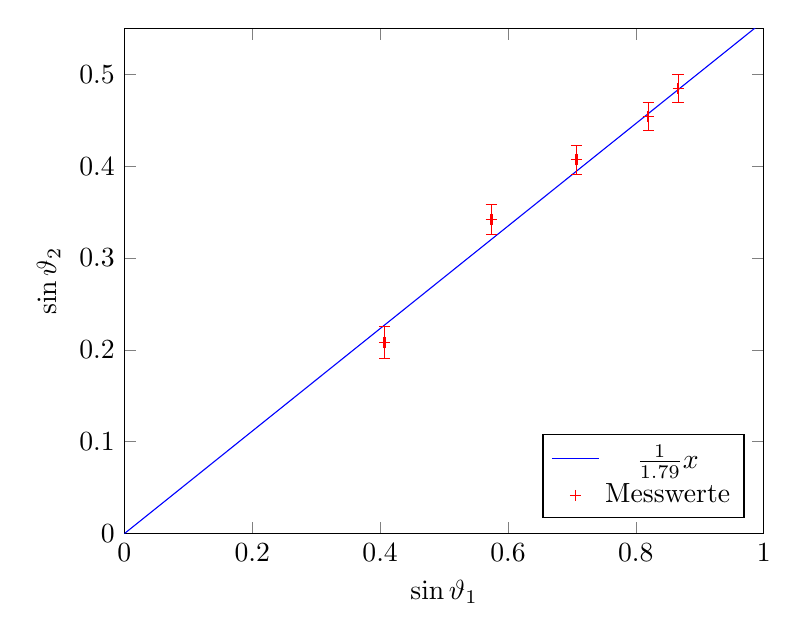
\begin{tikzpicture}
\begin{axis}[xmin = 0, ymin = 0, xmax = 1,
	legend pos = south east, width = .8\textwidth, height = 8cm,
	xlabel = $ \sin\vartheta_1 $,
	ylabel = $ \sin\vartheta_2 $]
	
	\addplot+[no marks, ] {1/1.7924933055*x};
	\addplot+[mark = +,only marks, error bars/.cd, x dir = both, x explicit, y dir=both, y explicit] table[x=x,y=y, x error = xerr, y error = yerr] {
x	y	xerr	yerr
0.4067366431	0.2079116908	0.0015944376	0.0170718962
0.5735764364	0.3420201433	0.00142969	0.0164007302
0.7071067812	0.4067366431	0.0012341341	0.0159443761
0.8191520443	0.4539904997	0.0010010797	0.0155509975
0.8660254038	0.4848096202	0.0008726646	0.0152649936
};
\legend{{$ \frac{1}{\num{1.79}}x $}, Messwerte}
\end{axis}
\end{tikzpicture}
\caption{Sinus des Ausfallwinkels gegen Sinus des Einfallwinkels aufgetragen}
\label{fig:n}
\end{figure}


\subsection{Totalreflexion}
Um mit Hilfe des PVC-Halbzylinders eine Totalreflexion zu erzeugen wird der Sender so ausgerichtet, dass dieser  auf die runde Oberfläche strahlt. Diese Strahlen werden gebrochen und propagieren durch den Halbzylinder.
Wenn die Mikrowellen auf die Grenzfläche zwischen PCV-Halbzylinder und Luft treffen $ n_{PVC}>n_{Luft} $, wird der transmittierende Strahl total reflektiert, wenn der Sender im richtigen Winkel auf den Halbzylinder strahlt.
Wird nun der zweite PVC-Halbzylinder in die nah genug an den Ersten gebracht, so entsteht eine frustrierte Totalreflexion.
Die Stärke dieser frustrierte Totalreflexion nimmt mit dem Abstand der Halbzylinder voneinander exponentiell ab. Dies lässt sich in Abbildung \ref{fig:frust} nachvollziehen.
%(hier Grafik einfügen)
\begin{figure}[H]
\centering
\includegraphics[width=0.9\linewidth]{./diagramme/frust_totalr_ohne_titel}
\caption{Gemessene Spannung gegen Lückenbreite aufgetragen}
\label{fig:frust}
\end{figure}

\subsection{Braggsche Reflektion}
In diesem Versuch soll die Gitterkonstante eines Gitters aus Metallkugeln aus der Bragg-Reflektion bestimmt werden. Dazu wird das Planetengetriebe des Versuchsaufbaus fixiert, so dass der Einfallwinkel immer dem Ausfallwinkel entspricht. Dann werden die möglichen Reflektionswinkel abgefahren und Maxima gesucht. Da für die Positionen der Maxima \eqref{eq:brag} bekannt ist, lässt sich damit die Gitterkonstante bestimmen.\\
Wir erhielten Maxima unter den Winkeln \SIlist{6.5+-1; 19+-1; 29+-1; 58.5 +-1}{\degree}. Durch umstellen von \eqref{eq:brag} erhält man daraus für $ \frac{d}{n} $ die folgenden Werte: \\
\sisetup{table-figures-integer=2, table-figures-decimal=2, table-number-alignment=center, table-figures-uncertainty = 2}
\begin{tabular}{r|S[table-figures-decimal=1]S[table-figures-decimal=1]SS}
Winkel in \si{\degree} & 6.5+-1 & 19+-1 & 29+-1 & 58.5 +-1 \\
$ \frac{d}{n} $ in \si{\centi\meter} & 14(5) & 4.8(5) & 3.21(21) & 1.83(5)
\end{tabular}
Mir ist keine Möglichkeit bekannt, aus diesen Werten die Gitterkonstante logisch zu schlussfolgern.
\newpage
\section{Diskussion} 
\subsection{Strahldivergenz}
Es war bei uns gut zu erkennen, dass sich um den fokusierten, intensivsten Teil der Strahlung in der Mitte ein Kegel, beziehungsweise in der zweidimensionalen Projektion ein Dreieck, bildet, in dem die Intensität nach außen hin abnimmt. Jedoch zeigte sich die Symmetrie die anzunehmen ist nur bedingt. Dies liegt aber wahrscheinlich zum größten Teil an der schlechten Reproduzierbarkeit der Messwerte. Die am Sensor gemessene Spannung unterlag starken Schwankungen so dass genaue Aussagen nur schwer möglich sind. 
\subsection{Wellenlänge}
Wir haben eine Wellenlänge von etwa \SI{3.123}{\centi\meter} ermittelt. Somit liegt die Frequenz der Mikrowellen bei etwa $ f = \SI{10}{\giga\hertz} $. Das ist in etwa die doppelte Frequenz von WLAN im \SI{5}{\giga\hertz}-Band. Die Resonanzfrequenz von Wassermolekülen liegt dagegen etwa doppelt so hoch bei \SI{22}{\giga\hertz}. Die Strahlenquelle passt gut in den definierten Bereich der Mikrowellenstrahlung.\\
Der Versuch hat im Grunde eine Möglichkeit gezeigt, mit einfachen Mitteln eine elektromagnetische Welle zu charakterisieren. Auch die Genauigkeit kann für viele Anwendungen ausreichen. Dass in den Knotenpunkten keine Nullstellen sind ist auch kein Problem. Das der idealisierte Zusammenhang der vollständigen Auslöschung in den Knotenpunkten nicht in der Praxis zu sehen ist war zu erwarten. Dennoch konnten wir genug direkt nebeneinander liegende Minima finden, um die Wellenlänge zuverlässig zu bestimmen. 

\subsection{Brechung an PVC}
Bei diesem Versuch hat sich gezeigt, dass sich die Brechung von Mikrowellen an PVC analog zur im vorherigen Versuch und im Alltag beobachteten Lichtbrechung verhält. In Abbildung \ref{fig:n} ist gut zu sehen, dass wie von der Lichtbrechung bekannt, zwischen Sinus von Einfallwinkel und Ausfallwinkel ein proportionales Verhältnis besteht. Der Proportionalitätsfaktor ergibt sich dabei aus den Brechungsindizes. \\
Die bei diesem Versuch erreichte Genauigkeit ist jedoch relativ gering. Die Ursache liegt wohl darin, dass, wie auch in jedem anderen Versuchsteil, die Spannung nicht sehr gut bestimmen lässt. Dies macht es nicht möglich das Maximum und somit den genauen Ausfallwinkel mit geringer Unsicherheit zu bestimmen. Dies ist auch in Abbildung \ref{fig:n} zu erkennen. Während die Unsicherheit des einfallenden Winkels am Diagramm kaum erkennbar sind, decken die Fehlerbalken des ausfallenden Winkels verhältnismäßig große Bereiche ab.

\subsection{Totalreflektion}
Qualitativ konnten wir die evaneszente Welle nachweisen. Auch ist in Abbildung \ref{fig:frust} die Intensitätsschwächung mit zunehmender Spaltbreite qualitativ erkennbar. Jedoch ließ sich der exponentielle Zusammenhang nicht belegen. \\
Das quantitativ Vernünftige Ergebnisse hier nicht möglich waren ist nicht nur eine Folge der problematischen Spannungsmessung. Es kam in diesem Versuchsteil erschwerend hinzu, dass das genaueste Messgerät zur Abstandsmessung, dass zur Verfügung stand ein Maßband mit Millimetermarkierungen war. Jedoch spielt sich der Effekt auf einem Abstandsbereich bis \SI{2}{\centi\meter} ab. In diesem Bereich wären Messungen mit einem Messschieber deutlich genauer und zuverlässiger. 

\subsection{Bragg Winkel}
Die in diesem Versuch erfassten Messwerte sind im Grunde unbrauchbar. Wir haben zur Referenz die Gitterkonstante mit einem Maßband am Gitter direkt gemessen. Wir erhielten dabei eine Gitterkonstante von etwa \SI{3.825}{\centi\meter}. Dieser Wert ist jedoch mit unseren Messwerten nicht vereinbar. Er würde bei den Winkeln \SIlist{6.5;19}{\degree} eine natürliche Zahl zwischen \numlist{0;1} voraussetzen. Das heißt, dass der Versuch stark störanfällig ist, da auch durch andere Effekte Maxima auftreten können. Zudem konnten wir feststellen, dass die andere Gruppe, die zeitgleich mit uns den Versuch durchgeführt hat, unterschiedliche Werte erhalten hat, abhängig davon ob wir die Strahlenquelle aktiv hatten.